\documentclass[output=paper]{langscibook}
\ChapterDOI{10.5281/zenodo.15148188}
\author{Darya Kavitskaya\orcid{}\affiliation{University of California, Berkeley} and Florian Wandl\orcid{}\affiliation{University of Zurich} }
\title{Preservation and loss of a rare contrast: Palatalization of rhotics in Slavic}
\abstract{This chapter discusses the rise and development of the cross-linguistically rare contrast between plain and palatalized rhotics in Slavic. We observe that the contrast, which developed as a result of \textit{yod}-palatalization (jotation) in Common Slavic, has been preserved only in languages which introduced additional palatalized rhotics as a result of palatalization before front vowels. We argue that this correlation is not coincidental, but that the functional load of the contrast as well as its integration into a correlation of plain and palatalized consonants were instrumental for the preservation of the rare contrast. However, only a few of the languages which had originally preserved the contrast still have palatalized rhotics today. In others we find either loss or stabilization of the contrast by altering the palatalized rhotic. The proposed analysis sheds light on the factors potentially involved in the development of rare contrasts.

\keywords{palatalization, phonological contrast, functional load, rhotics, Slavic}
}
\IfFileExists{../localcommands.tex}{
  \addbibresource{../localbibliography.bib}
  \usepackage{tabularx, multicol, multirow, longtable}
\usepackage{url}
\urlstyle{same}

\usepackage{orcidlink}
\definecolor{orcidlogocol}{cmyk}{0,0,0,1}
\RenewDocumentCommand{\LinkToORCIDinAffiliations}{ +m }
  {%
    \orcidlink{#1}\,%
  }
\SetupAffiliations{orcid placement=before}

\usepackage{siunitx}
\sisetup{detect-weight=true, detect-family=true, group-digits=none}

\usepackage{mathtools}
\usepackage{langsci-optional}
\usepackage{langsci-lgr}
\usepackage{langsci-gb4e}

\usepackage{stmaryrd}
\usepackage[capitalize]{cleveref}
\babelfont[macedonian]{rm}[Language=Macedonian,ItalicFont=LibertinusSerif-Italic.otf]{LibertinusSerif-Regular.otf}
\usepackage{eqparbox}
\usepackage[autostyle]{csquotes}
\usepackage[linguistics]{forest}

\usetikzlibrary{positioning, matrix}
\usepackage[glosses,inline]{leipzig}
\PassOptionsToPackage{xindy,toc,nopostdot}{glossaries}
\usepackage{glossary-inline}
\setglossarystyle{inline}
\makeglossaries

\usepackage{phonrule}
\usepackage{threeparttable}


\usepackage{textcomp,gensymb}


\usepackage[preservefont]{tipauni}

\usepackage[normalem]{ulem}

\usepackage{enumitem} %so lists aren't ugly
	
\usepackage{threeparttable}	%allows tables with tablenotes. note marks: †‡
	\makeatletter 
	\g@addto@macro\TPT@defaults{\footnotesize} 
	\makeatother

\usepackage{colortbl}
	\definecolor{Pink}{rgb}{0.96, 0.76, 0.76} 
	\definecolor{PaleBlue}{rgb}{0.67, 0.9, 0.93}
	\definecolor{carolinablue}{rgb}{0.6, 0.73, 0.89}
	\definecolor{goldenyellow}{rgb}{1.0, 0.87, 0.0}
	\definecolor{Orange}{rgb}{1.0, 0.66, 0.07}
	\definecolor{puce}{rgb}{0.8, 0.53, 0.6}
	\definecolor{turquoisegreen}{rgb}{0.63, 0.84, 0.71}


% add all extra packages you need to load to this file
\usepackage{langsci-textipa}
\usepackage{vowel}
\usepackage{textgreek}

% \usepackage{langsci-branding}
% \usepackage{subcaption}
\usepackage{subfigure}

\usepackage{tabto}


\usetikzlibrary{tikzmark}
\usepackage{pgfplots}


\newfontfamily\tibetan{NotoSerifTibetan-Regular.ttf}
\usepackage{langsci-branding}
\usepackage{hyphenat}

\usepackage{accents}

  \renewcommand{\lsChapterFooterSize}{\footnotesize}

\makeatletter
\let\thetitle\@title
\let\theauthor\@author
\makeatother

\newcommand{\togglepaper}[1][0]{
   \bibliography{../localbibliography}
   \papernote{\scriptsize\normalfont
     \theauthor.
     \titleTemp.
     To appear in:
     Natalia Kuznetsova, Cormac Anderson \& Shelece Easterday (ed.).
     Rarities in phonetics and phonology.tex.
     Berlin: Language Science Press. [preliminary page numbering]
   }
   \pagenumbering{roman}
   \setcounter{chapter}{#1}
   \addtocounter{chapter}{-1}
}

\newbool{bookcompile}
\booltrue{bookcompile}
\newcommand{\bookorchapter}[2]{\ifbool{bookcompile}{#1}{#2}}

\newcommand{\textarab}[1]{\RL{\arabicfont #1}}

\newcommand\mb[1]{\eqparbox[t]{examples}{#1}\hspace{1em}}
\newcommand\mbi[1]{\mb{#1}}
\newcommand{\twe}[3]{\mbi{#1}\eqparbox[t]{orths}{\emph{#2}}\hspace{1em}`#3'\hspace{1em}} % three-way example
\providecommand\glottocode[1]{[\href{https://glottolog.org/resource/languoid/id/#1}{#1}]}
\newcommand{\phonreal}[1]{\ensuremath{\llbracket}#1\ensuremath{\rrbracket}}

\DeclareRobustCommand\dash{\unskip\nobreak\thinspace\textendash\allowbreak\thinspace\ignorespaces}

\forestset{minus/.style={edge label={node[midway, left] {\ensuremath{-}\hspace*{2mm}}}},
plus/.style={edge label={node[midway, right] {\hspace*{2mm}\ensuremath{+}}}}}
\providecommand\ipa[1]{#1}


\newcommand{\tone}[1]{\textsuperscript{#1}}

\newcommand{\orthog}[1]{\textit{#1}}
\newcommand{\gloss}[1]{`#1'}

\newcommand{\glottolog}[1]{\texttt{\href{https://glottolog.org/resource/languoid/id/#1}{#1}}}

\newcolumntype{O}{>{\itshape }l<{}}
\newcolumntype{G}{>{`}l<{'}}

\newcounter{tabsubcounter}
\newcommand{\tablecounter}{\setcounter{tabsubcounter}{0}}
\newcommand{\TC}{\stepcounter{tabsubcounter}\alph{tabsubcounter}.}

\usetikzlibrary{chains,positioning,calc,decorations.markings}
\tikzset{
	seg/.style={text height=0.6em, text depth=0.3em},
	moraic-structure/.style={xscale=0.6,yscale=1.1, text height=0.65em,text depth=0.25em},
 }

%05_Culhane_Edwards
%%%%%%%%%%%%%%%%%%%%%%%%%%%%%%%%
%%	Symbols and Characters  	%%
%%%%%%%%%%%%%%%%%%%%%%%%%%%%%%%% αβσµ

\newcommand{\tl}{\char`~}						%middle tilde ~
\renewcommand{\Q}{\textquotesingle}		%straight apostrophe444
\newcommand{\ra}{→} 								%right arrow ->
\newcommand{\0}{∅} 									%zero symbol
\newcommand{\gap}{\textunderscore} 	%underscore
%\renewcommand{\j}{ʤ}								%dezh digraph
\newcommand{\syll}{σ}								%lowercase sigma medial form
\newcommand{\wrd}{ω}								%lowercase omega
\newcommand{\ft}{φ}									%lowercase phi
\newcommand{\gw}{gʷ}								%g with superscript w
\newcommand{\B}{β}									%voiced bilabial fricative
\newcommand{\hp}{\hphantom}					%space equal to width of argument
\newcommand{\it}{\textit}	%italics

%%%%%%%%%%%%%%%%%%%%%%%%%%%%%%%%
%%	Font Styles & Formatting	%%
%%%%%%%%%%%%%%%%%%%%%%%%%%%%%%%%

\definecolor{DarkBlue}{RGB}{0,0,130}										%dark blue colour
% \newcommand{\ve}[1]{\textcolor{DarkBlue}{\textit{#1}}}	%vernacular text
\newcommand{\ve}[1]{{\textit{#1}}}	%vernacular text
\definecolor{DarkRed}{RGB}{150,0,0}											%dark red colour
% \newcommand{\tbr}[1]{\textcolor{DarkRed}{\textbf{#1}}}	%Bold red text
\newcommand{\tbr}[1]{{\textbf{#1}}}	%Bold red text
%\renewcommand{\it}{\textit}																%italics
\newcommand{\tsc}{\textsc}															%small caps
\newcommand{\sub}{\textsubscript}												%subscript
\newcommand{\su}{\textsuperscript}											%superscript

%%%%%%%%%%%%%%%%%%%%%%%%%%%%%%%%%%%%%%%%%%%%%%%%%%%%
%% Tables %% Tables %% Tables %% Tables %% Tables %%
%%%%%%%%%%%%%%%%%%%%%%%%%%%%%%%%%%%%%%%%%%%%%%%%%%%%

% \newcommand{\mc}{\multicolumn}									%multicolumn
% \newcommand{\st}[1]{\setlength{\tabcolsep}{#1}}	%reduce column width in tables
%
%%%%%%%%%%%%%%%%%%%%%%%%%%%%%%%%
%%    Cross   References      %%
%%%%%%%%%%%%%%%%%%%%%%%%%%%%%%%%

% \def\Plus{\texttt{+}}
% \def\Minus{\texttt{-}}
% \newcommand{\GS}{ʔ}
% \def\SH{ʃ}
% \newcommand{\TSH}{ʧ}
% \def\ZH{ʒ}
% \def\DZH{ʤ}
% \def\:{ː}
% \def\UP{\textsuperscript}
% \def\rs{ʂ}
% \newcommand{\rn}{ɳ}
% \def\rt{ʈ}
% \def\tllr{ɺ}
% \newcommand{\Bb}{β}
% \def\Eps{ɛ}
% \def\Oo{ɔ}
% \def\Gm{ɣ}
% \def\NG{ŋ}
% \def\barU{ʉ}
\newcommand{\CM}{\ding{51}}
\newcommand{\XM}{\ding{53}}
% \newcommand{\tap}{ɾ}
% \def\darkL{ɫ}
% \def\schwa{ə}
%
% \def\BUL{\textbullet}


%%%%%%%%%%%%%%
%					%
%	Secondaries		%
%					%
%%%%%%%%%%%%%%
%	Post
\newcommand{\Post}[2]{#1\textsuperscript{#2}}
%	Pre
\newcommand{\Pre} [2] {\textsuperscript{#1}#2}
%	Undertilde
\newcommand{\utilde}[1]{\ensuremath{\smash{\underset{\mathclap{\sim}}{\text{#1}}}}}
%	Devoiced
% \newcommand{\VCLS}[1]{\textsubring{#1}}
%%%%%%%%%%%
%				%
%	Definitions		%
%	Markup		%
%				%
%%%%%%%%%%%
% \def\->{$\rightarrow$}
% \def\__{\underline{\hspace{1em}}}
\def\NoPoss{\cellcolor{gray!30}}

\newcommand{\VOICELESS}{\textsc{voiceless}}
\newcommand{\VOICED}{\textsc{voiced}}
\newcommand{\tablenote}[2][1]{\parbox{#1\textwidth}{\footnotesize\raggedright #2}}

\newcommand{\appref}[1]{Appendix~\ref{#1}}
\renewcommand{\sectref}[1]{Section~\ref{#1}}


\newcommand{\dobuibox}[5]{#1\\[-1.1em]
\hspace*{-.8cm}
 \begin{tabularx}{.9\textwidth}{@{}lQQ@{}}
       &  {oral} &  {nasal} \\
       \midrule
     {controlled} &\parbox[t]{4cm}{\raggedright  #2} & \parbox[t]{4cm}{\raggedright #3} \\
     \tablevspace
     {ballistic} &\parbox[t]{4cm}{\raggedright  #4} & \parbox[t]{4cm}{\raggedright  #5} \\
 \end{tabularx}
}

\newfontfamily\VdottildeFont{LibertinusVdottilde.otf}

\newcommand{\Vdottilde}{{\VdottildeFont V̰̣}}

% \renewcommand{\keywords}[1]{\textbf{#1}}
 
  %% hyphenation points for line breaks
%% Normally, automatic hyphenation in LaTeX is very good
%% If a word is mis-hyphenated, add it to this file
%%
%% add information to TeX file before \begin{document} with:
%% %% hyphenation points for line breaks
%% Normally, automatic hyphenation in LaTeX is very good
%% If a word is mis-hyphenated, add it to this file
%%
%% add information to TeX file before \begin{document} with:
%% %% hyphenation points for line breaks
%% Normally, automatic hyphenation in LaTeX is very good
%% If a word is mis-hyphenated, add it to this file
%%
%% add information to TeX file before \begin{document} with:
%% \include{localhyphenation}
\hyphenation{
    af-fri-cates
    al-ve-o-pal-a-tal
    Ama-nu-ban
    Ara-wak-an
    Árna-son
    Ber-ber
    can-di-dates
    Cam-er-oon
    Chi-nan-tec
    Chir-ko-va
    Crai-o-ve-a-nu
    di-chot-o-my
    Ec-ua-do-rian
    Ec-ua-dor
    elec-tro-glot-to-gra-phy
    Faro-ese
    Ike-ma
    Kuznet-sova
    Mes-kwa-ki
    Mio-ma-fo
    mono-mor-aic
    Ne-ca-xa
    Oto-man-gue-an
    par-a-digm
    post-as-pi-rat-ed
    post-as-pi-ra-tion
    pre-as-pi-rat-ed
    pre-as-pi-ra-tion
    pros-o-dic
    pros-o-dies
    re-con-struc-table
    Sheh-ret
    Svan-tes-son
    Ta-ras-can
    Tórs-havn
    Ural-ic
    epen-the-sis
    Anin-dil-yak-wa
    Mi-nyag
    Na-ka-ma
}

\hyphenation{
    af-fri-cates
    al-ve-o-pal-a-tal
    Ama-nu-ban
    Ara-wak-an
    Árna-son
    Ber-ber
    can-di-dates
    Cam-er-oon
    Chi-nan-tec
    Chir-ko-va
    Crai-o-ve-a-nu
    di-chot-o-my
    Ec-ua-do-rian
    Ec-ua-dor
    elec-tro-glot-to-gra-phy
    Faro-ese
    Ike-ma
    Kuznet-sova
    Mes-kwa-ki
    Mio-ma-fo
    mono-mor-aic
    Ne-ca-xa
    Oto-man-gue-an
    par-a-digm
    post-as-pi-rat-ed
    post-as-pi-ra-tion
    pre-as-pi-rat-ed
    pre-as-pi-ra-tion
    pros-o-dic
    pros-o-dies
    re-con-struc-table
    Sheh-ret
    Svan-tes-son
    Ta-ras-can
    Tórs-havn
    Ural-ic
    epen-the-sis
    Anin-dil-yak-wa
    Mi-nyag
    Na-ka-ma
}

\hyphenation{
    af-fri-cates
    al-ve-o-pal-a-tal
    Ama-nu-ban
    Ara-wak-an
    Árna-son
    Ber-ber
    can-di-dates
    Cam-er-oon
    Chi-nan-tec
    Chir-ko-va
    Crai-o-ve-a-nu
    di-chot-o-my
    Ec-ua-do-rian
    Ec-ua-dor
    elec-tro-glot-to-gra-phy
    Faro-ese
    Ike-ma
    Kuznet-sova
    Mes-kwa-ki
    Mio-ma-fo
    mono-mor-aic
    Ne-ca-xa
    Oto-man-gue-an
    par-a-digm
    post-as-pi-rat-ed
    post-as-pi-ra-tion
    pre-as-pi-rat-ed
    pre-as-pi-ra-tion
    pros-o-dic
    pros-o-dies
    re-con-struc-table
    Sheh-ret
    Svan-tes-son
    Ta-ras-can
    Tórs-havn
    Ural-ic
    epen-the-sis
    Anin-dil-yak-wa
    Mi-nyag
    Na-ka-ma
}
 
  \togglepaper[14]%%chapternumber
}{}

\begin{document}
\maketitle 
%\shorttitlerunninghead{}%%use this for an abridged title in the page headers
% ATTENTION: Diacritics on the following phonetic characters might have been lost during conversion: {'ɔ', 'ɛ', 'ɪ'}




\section{Introduction}
\label{sec:kavitskaya:1}
In the spirit of the volume, this chapter addresses a rare contrast between plain and palatalized rhotics attested in several Slavic languages, such as Russian (russ\-1263), Ukrainian (ukra1253), Eastern Bulgarian (Bulgarian: bulg1262), Upper Sorbian (uppe1395), and Lower Sorbian (lowe1385), e.g. Ukr /rad/ ‘glad’ : /rʲad/ ‘row’.\footnote{The list of abbreviations can be found at the end of the chapter.}  In other Slavic languages, the contrast is either absent, as in Slovenian (slov1268) and Bosnian/Croatian/Serbian (sout1528), or a different type of contrast is present as a result of a shift in the place or manner of articulation of the originally palatalized member of the contrastive pair /r/ : /rʲ/. For instance, in Czech (czec1258), the contrast in rhotics is preserved as /r/ : /r̝/ (cf. *\textit{marjā} ‘sea-\textsc{gen.sg}’ > \textit{mo}[r̝]\textit{a}), and in Polish (poli1260) the sound change went one step further, with the original palatalized rhotic losing both its rhoticity and its palatalization (cf. *\textit{marjā > mo}[ʒ]\textit{a}).\footnote{In our reconstruction of PSl forms we follow \citet{Holzer1995,Holzer2003}.}

Provided that the contrast is phonetically unstable and typologically rare (see the discussion in \sectref{sec:kavitskaya:2}), we explore the reasons for its preservation in Slavic. It has been proposed that the palatalization contrast is preserved due to various phonetic stabilization strategies found in Slavic languages (\citealt{IskarousKavitskaya2018}). However, we find that the historical development of the palatalization system in Slavic can shed light on how and why the contrastive palatalization of rhotics was preserved. Secondary palatalization of rhotics first arose through an early sound change of \textit{yod}-palatalization (jotation), and more palatalization contexts were introduced later in individual Slavic languages. We show that the /r/ : /rʲ/ contrast has been preserved only in those Slavic languages that acquired additional palatalization contrasts in positions other than the jotation context. We suggest that this correlation is not coincidental and that, in addition to the phonetic pressures, there are also functional pressures, such as the functional load of the contrast and the structure of the consonant inventory, that are crucial for the contrast preservation (\citealt{Martinet1952,Hockett1967,WedelEtAl2013b,WedelEtAl2013a}).

We address the question of the rarity of the contrast in \sectref{sec:kavitskaya:2}. \sectref{sec:kavitskaya:3} discusses the sources of the Slavic palatalized rhotics, and \sectref{sec:kavitskaya:4} addresses the issues of preservation and loss of these segments in Slavic. \sectref{sec:kavitskaya:5} will turn to the functional explanation of the contrast preservation, followed by the discussion of the phonetic considerations in the preservation and loss of palatalized rhotics, as well as some aspects of their acquisition.

\section{Rhotics and palatalization}
\label{sec:kavitskaya:2}
The phonetic secondary palatalization of consonants is widely attested in the world’s languages, but phonological, that is, contrastive secondary palatalization is less typologically common (\citealt{Bhat1978,Stadnik2002,Bateman2011,KrämerUrek2016}). For example, in a balanced 100 language sample, only 7 languages show a secondary palatalization contrast \citep{Easterday2017}. The contrastive palatalization of rhotics specifically is even more rare (\citealt{Hall2000,Żygis2005}; \citealt{Jaworski2018}: 47-50; \citealt{NikolaevGrossman2020}: 431). It is attested only in a handful of languages, e.g., according to PHOIBLE (\citealt{MoranMcCloy2019}), palatalized trills occur in 28 (1.3\%) languages in their database of 2186 languages, and palatalized taps occur in 18 (0.8\%) languages in the database. LAPSyD (\citealt{MaddiesonEtAl2016}) supports these results: only 13 languages out of 806 (1.6\%) have palatalized rhotics.\footnote{Note that non-palatalized rhotics are much more common: for instance, 247 languages out of 806 (31\%) in LAPSyD have segments that are classified as alveolar trills.} For instance, the contrastive secondary palatalization of rhotics is present in Irish, Japanese, Marshallese, Tundra Nenets, and, importantly for us here, in several Slavic languages.

Although phonemic trilled rhotics are by no means rare, phonetically, they commonly exhibit a number of non-trilled allophones, such as taps, approximants, or fricated approximants (see \citealt{Colantoni2006,Wiese2001,VerstraetenVelde2001,Solé2002,RecasensEspinosa2007,Żygis2005,JaworskiGillian2011}; among others). Specifically in Slavic, while the rhotics are usually classified as trills, they are rarely truly trilled phonetically. In a detailed study, \citet[113-120]{Jaworski2018} reports the following allophones of /r/ in Slavic: [r], [r̞], [ɾ], [ɾᶾ], [ɹ], [ɹ̞]. In Russian, the non-palatalized /r/, traditionally described as a trill, is most commonly realized as a tap and quite often surfaces as an approximant (\citealt{KavitskayaEtAl2009,IskarousKavitskaya2010,Jaworski2018}).\footnote{A reviewer raises a question of whether Slavic rhotics can be characterized phonologically as trills, given the number of different allophones of these segments. While the resolution of this question is far from straightforward, there are several arguments for treating the Slavic /r/ as an underlying trill. First, the speakers of Slavic languages pronounce this segment as a trill in isolation. Second, the phonological behavior of the rhotic argues for the trill analysis: taps are mostly attested intervocalically, voiceless allophones of the /r/ are attested word-finally and before voiceless consonants, approximants are common post-vocalically, while there is a greater likelihood of trills occurring word-initially (\citealt{IskarousKavitskaya2010}). In regard to the diachronic data, all attested reflexes of the PSl \textit{*r} can be traced back to a trill rather than to any other rhotic.}

Many proposals have addressed the incompatibility of rhotics and palatalization. It has been argued that the rarity of the palatalization contrast in rhotics is due to the conflicting articulatory and/or aerodynamic demands on palatalization and rhotics in general and trilled rhotics in particular. While palatalization involves tongue dorsum raising, rhotics require tongue root backing (see \citealt{Kochetov2005,Hall2000,IskarousKavitskaya2010,Jaworski2018}; among others). To illustrate this, \figref{fig:kavitskaya:1} shows that in Russian, the tongue dorsum is raised towards the palate in the [rʲ] in comparison with the plain [r]. The comparison of the plain [r] and [d] in Figures 1 and 2 shows that both of these require tongue root backing (note that [d] is velarized in Russian). Finally, there is no tongue backing in the palatalized [dʲ], as expected (\figref{fig:kavitskaya:2}). However, tongue backing is still present in the palatalized [rʲ], even though not as strongly as for the plain [r] (\figref{fig:kavitskaya:1}).

\begin{figure}
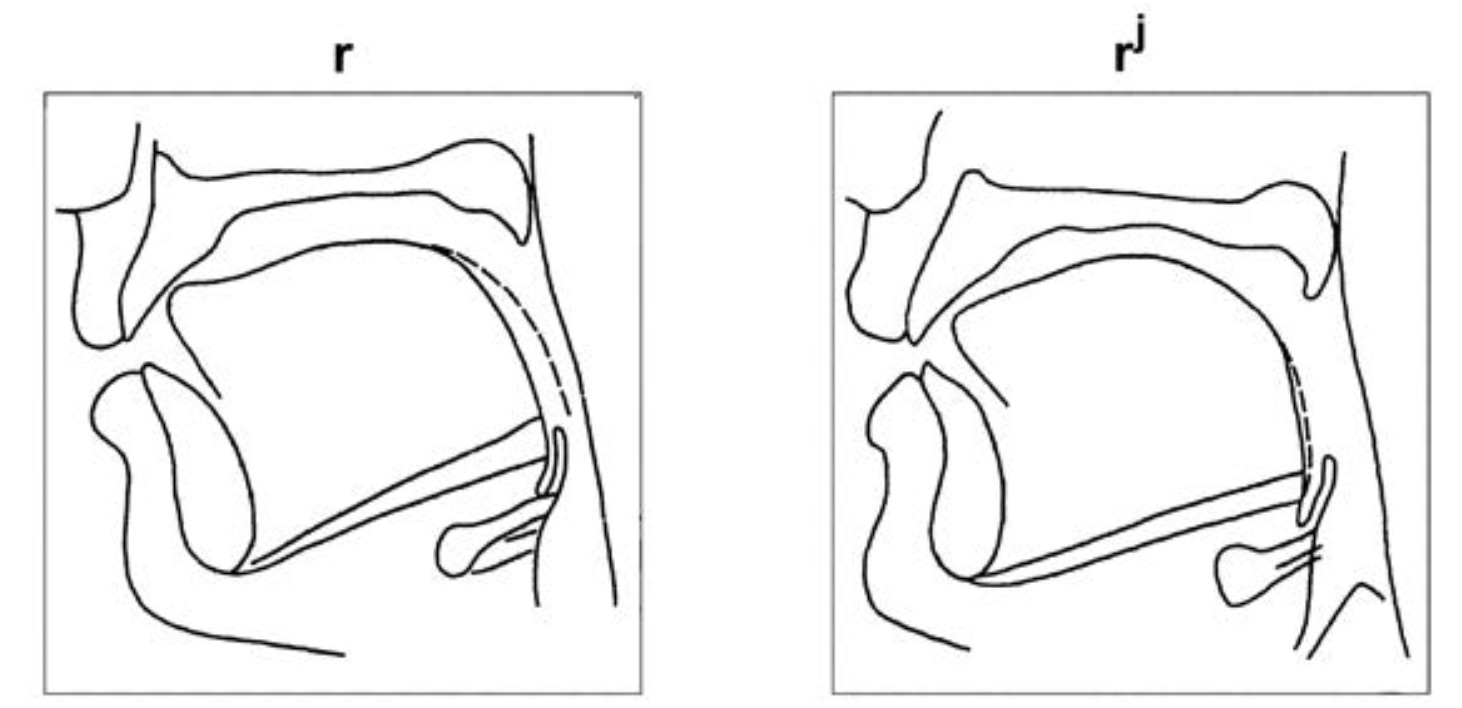
\includegraphics[width=\textwidth]{figures/a14KavitskayaWandl-img001.jpg}
\caption{\label{fig:kavitskaya:1} Tracings of the articulatory structures for [r] and [rʲ] in Russian (\citealt{IskarousKavitskaya2018}, adapted from \citealt{Bolla1981})}
\end{figure}

\begin{figure}
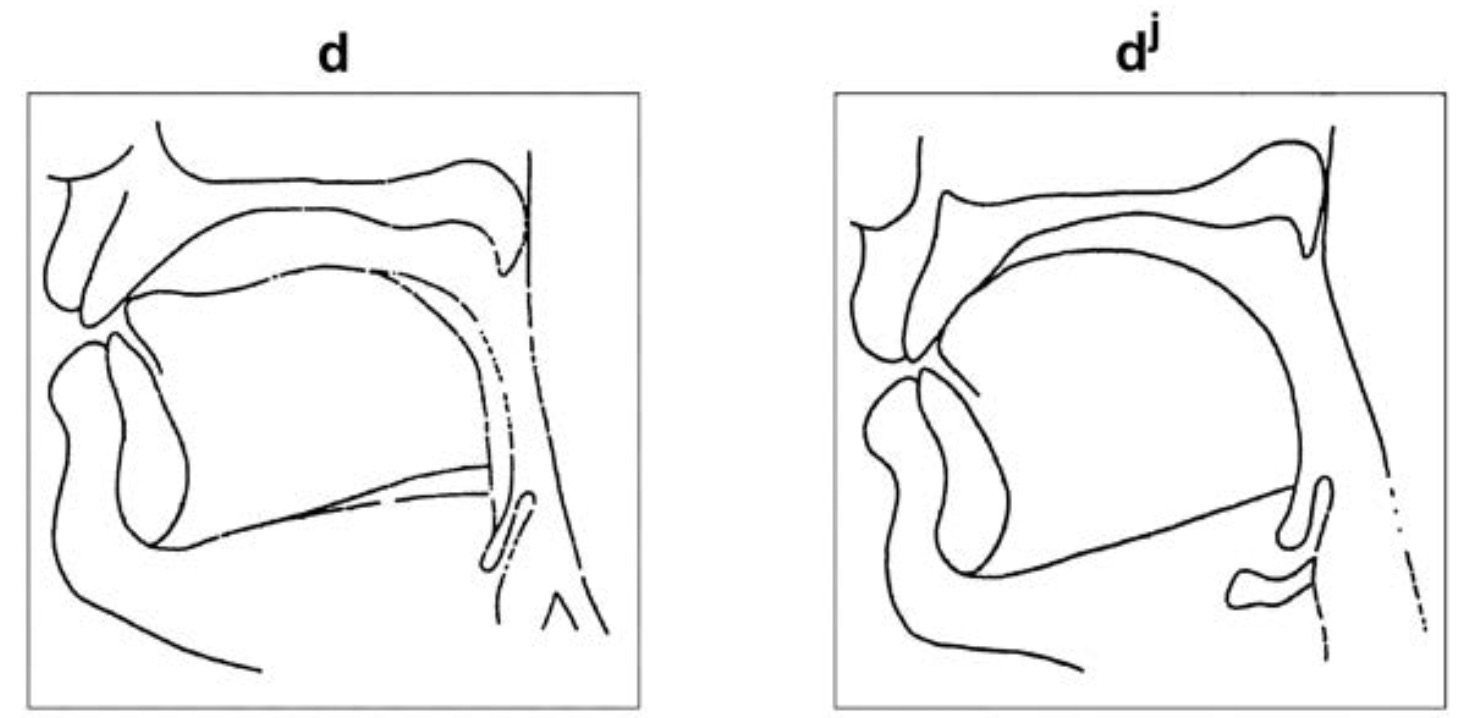
\includegraphics[width=\textwidth]{figures/a14KavitskayaWandl-img002.jpg}
\caption{\label{fig:kavitskaya:2} Tracings of the articulatory structures for [d] and [dʲ] in Russian (\citealt{IskarousKavitskaya2018}, adapted from \citealt{Bolla1981})}
\end{figure}

Trilling has an additional detrimental effect on palatalization. It has been suggested that this is due to the articulatory constraints on the production of palatalized trills, which result in conflicting aerodynamic demands on the tongue dorsum (\citealt{Kavitskaya1997,LadefogedMaddieson1996}: 221; \citealt{KavitskayaEtAl2009,Proctor2011}; among others). While palatalization requires fronting of the tongue into the palatal region of the mouth, trilling depends on tongue retraction in order to stabilize the tongue dorsum, which needs to be immobilized during the trilling in order not to inhibit the vibration of the tongue tip \citep{McGowan1992}. Alternatively, \citet{Howson2018} argues that the inconsistency between palatalization and trills is due to “the inability to create proper tongue stability and the constant movement towards a palatal target likely interferes with the aerodynamic conditions necessary to produce trilling” \citep[148]{Howson2018}. Whatever the reason is, it is evident that palatalized trills are phonetically unstable segments.

It has been proposed that the conflicting articulatory demands on palatalized rhotics are responsible for the elimination of /rʲ/ and thus for the loss of contrast in rhotics in several Slavic languages (\citealt{KavitskayaEtAl2009,Jaworski2018}). However, given its instability and rarity, it is remarkable that the contrast /r/ : /rʲ/ is attested in Slavic languages belonging to different subgroups, such as Russian and Ukrainian (East Slavic), Eastern Bulgarian (South Slavic), Upper Sorbian and Lower Sorbian (West Slavic), as illustrated in (\ref{bkm:Ref102914657}).


\ea \label{bkm:Ref102914657}Contrastive /r/ : /rʲ/ pairs in Slavic
  \ea Russian\\
      \textit{rad}   ‘glad’  :  \textit{rʲad}   ‘row’
  \ex Ukrainian\\
      \textit{rad}   ‘glad’  :  \textit{rʲad}   ‘row’
  \ex Eastern Bulgarian\\
      \textit{gora}   ‘forest’  :  \textit{gorʲa}   ‘burn’
  \ex Upper Sorbian\\
      \textit{ʀad}   ‘glad’  :  \textit{ʀʲad}   ‘row’
  \z
\z

In the remainder of the chapter we will first discuss the emergence and the development of palatalized rhotics in Slavic and then address the factors that influenced the preservation and loss of the /r/ : /rʲ/ contrast in the individual Slavic languages.

\section{Sources of palatalized rhotics in Slavic}
\label{sec:kavitskaya:3}
There are two main sources of palatalized rhotics in Slavic: jotation and palatalization before front vowels. Jotation is the term used in Slavic linguistics to refer to a Common Slavic change that comprises the palatalization of consonants before \textit{j} (yod palatalization) and the subsequent loss of the glide that triggered palatalization. Jotation affected all coronal consonants, that is, /s, z, t, d, l, n, r/, including the laterals which have been introduced as a result of \textit{l}{}-epenthesis between labials and *\textit{j}, cf. PSl *\textit{pj}, *\textit{bj}, *\textit{mj}~> *\textit{plj}, *\textit{blj}, *\textit{mlj}.\footnote{Sequences of velar obstruents and yod had most probably been eliminated by the pre-Proto-Slavic First (regressive) Palatalization at the time when jotation took place. For more details on the jotation change in Slavic see \citet{Shevelov1964}, \citet[112-115]{Carlton1991}, and \citet{WandlKavitskaya2023}. A recent discussion of the Common Slavic velar palatalizations can be found in \citet{Wandl2020}.} Apart from rhotics, as a result of jotation all coronals underwent a change in the place of articulation, which in many cases was accompanied by a change in the manner of articulation. Thus, the Proto-Slavic sequences *\textit{sj} and *\textit{zj} are reflected as either [ʃ] and [ʒ], or [ʂ] and [ʐ] in attested Slavic, as shown in (\ref{bkm:Ref102736576}). The jotation reflexes of PSl *\textit{tj} and *\textit{dj} are shown in (\ref{bkm:Ref102464165}).


\ea \label{bkm:Ref102736576}Contemporary reflexes of PSl *\textit{sj} and *\textit{zj}
\ea PSl *\textit{nasjā} ‘load, burden’ > Ru \textit{no}[ʂ]\textit{a}, Cz \textit{nů}[ʃ]\textit{e}, Sln \textit{nó}[ʃ]\textit{a} ‘attire’
\ex PSl *\textit{kazjā} ‘skin, leather’ > Ru \textit{ko}[ʐ]\textit{a}, Cz \textit{ků}[ʒ]\textit{e}, Sln \textit{kó}[ʒ]\textit{a}
\z
\z

\ea \label{bkm:Ref102464165}Contemporary reflexes of PSl *\textit{tj} and *\textit{dj} in the continuants of PSl. *\textit{swajtjā} ‘candle’ and *\textit{medjā} ‘border’
\ea *\textit{tj} >   

    [ts]    Cz \textit{sví}[ts]\textit{e}, Slk \textit{svie}[ts]\textit{a}, Po \textit{świe}[ts]\textit{a}

  [tʃ]    Ru, BRu \textit{sve}[tʃ]\textit{á}, Ukr \textit{svi}[tʃ]\textit{á}, Sln \textit{své}[tʃ]\textit{a} 

  [tɕ]    BCS \textit{svijè}[tɕ]\textit{a} 

  [ʃt]    Bu \textit{sve}[ʃt]

  [c]    Mak \textit{sve}[c]\textit{a} 
\ex *\textit{dj} > 

   [z]    Cz \textit{me}[z]\textit{e}

  [dz]    Slk \textit{me}[dz]\textit{a}, Po \textit{mie}[dz]\textit{a}  

  [dʒ] > [ʒ]  Ru, Ukr, Bru \textit{me}[ʒ]\textit{á} 

  [dʑ]    BCS \textit{mè}[dʑ]\textit{a} 

  [j]    Sln \textit{mé}[j]\textit{a} 

  [ʒd]    Bu \textit{me}[ʒd]\textit{á}

  [ɉ]    Mak \textit{me}[ɉ]\textit{a} 
\z
\z

Laterals and nasals in the jotation context have either palatal or palatalized reflexes, e.g. PSl *\textit{valjā} > BCS \textit{vo}[ʎ]\textit{a} ‘will’ {\textasciitilde} Ru \textit{vo}[lʲ]\textit{a} ‘will’, PSl *\textit{vanjātī} > BCS \textit{vo}[ɲ]\textit{ati} ‘smell’ {\textasciitilde} Ru \textit{vo}[nʲ]\textit{at’} ‘stink’, or in the case of the lateral, may also have undergone depalatalization, e.g. Po \textit{wo}[l]\textit{a}, Cz \textit{vů}[l]\textit{e} ‘will’. Palatalized laterals and nasals occur in Russian, as can be seen from the examples above, and are also characteristic of the other East Slavic languages, Ukrainian and Belarusian (bela1254). However, the philological evidence from the East Slavic of the 11th and 12th centuries indicates that jotation originally induced a change in the place of articulation of laterals and nasals also in the East Slavic area. While laterals and nasals in the jotation context are marked orthographically in some manuscripts, secondarily palatalized laterals and nasals are not (see \citealt[21--22]{Kalnyn’1961}, \citealt{Živov1996}). Thus, Russian, Ukrainian, and Belarusian [lʲ] and [nʲ] in the jotation context developed from [ʎ] and [ɲ]. This suggests that a Common Slavic change in the place of articulation of consonants affected by jotation was not only typical for fricatives and plosives but also for laterals and nasals (\citealt{Stadnik2002}: 143-145; \citealt{WandlKavitskaya2023}).

Rhotics take a special position with regard to jotation among coronal consonants. Unlike fricatives, plosives, laterals, and nasals, rhotics do not occur in the palatal region, which rules out a change in the primary place of articulation. Therefore, as we argued elsewhere (\citealt{WandlKavitskaya2023}), the /r/ : /rʲ/ contrast is the only secondary palatalization contrast that can be reconstructed for Common Slavic (cf. also \citealt{Stadnik2002}: 144). With respect to the primary place of articulation, the Common Slavic rhotics can be safely reconstructed as apical trills. Of the major Slavic languages, only Upper Sorbian shows a uvular reflex, which is likely to be the result of language contact with German (see \citealt{Jaworski2018}: 80; \citealt{Howson2018}: 132). However, considering the high frequency of instances in which rhotics were realized as taps in contemporary Slavic, described by \citet{Jaworski2018} (see \sectref{sec:kavitskaya:2}), it seems reasonable to assume a tap allophone for a Common Slavic pre-stage. The contemporary reflexes of the Common Slavic pair /r/ : /rʲ/ resulting from jotation will be discussed in \sectref{sec:kavitskaya:4}.

The second, chronologically later change that introduced palatalized rhotics in Slavic is palatalization before front vowels.\footnote{See
  \citet{vanWijk1937,Gerovský1959,Koschmieder1959}, \citet[489--490]{Shevelov1964}, \citet[160]{Carlton1991}, \citet[167-176]{Stadnik2002} on the late dating of the secondary palatalization change.
}
It occurred after the beginning of the disintegration of Common Slavic. Hence, it is absent from BCS, Slovenian, and Macedonian (mace1250).\footnote{The situation may be different in some South Slavic dialects. For example, the palatalization of consonants is found in Macedonian dialects spoken in Greece (see \citealt{IvićEtAl1981}). We are grateful to Rafał Szeptyński for bringing these dialects to our attention. However, it should be noted that the dialects discussed by \citet{IvićEtAl1981} do not contradict our assumptions below.} Where palatalization before front vowels had occurred, it affected all consonants, although it should be noted that there may have been differences with regard to the vowels triggering palatalization in the individual languages (cf. the survey in \citealt{Carlton1991}: 157-164). Moreover, in some languages, secondary palatalization has been lost either as a result of depalatalization or due to changes in the place of articulation of the palatalized segments.\footnote{For more details on these developments, we refer the reader to specialized studies and the historical grammars of the individual Slavic languages (cf. \citealt{Kalnyn1961,Carlton1991,Stadnik2002}).}

What will be relevant for the discussion below is the phonologization of the secondarily palatalized consonants. Originally, secondary palatalization was an automatic process, which affected consonants before front vowels. Phonologization of the palatalized segments and thus the rise of the contrast /C/ : /Cʲ/ occurred only as a result of changes which rendered the palatalization triggers opaque, such as the backing or loss of the triggering vowel. As illustrated in (\ref{bkm:Ref59312723}) on the example of the Russian rhotics, denasalization and backing of the \textit{e}{}-like nasal vowel *\textit{ę} (most likely pronounced as [ɛ] or [\~{æ}]) to non-front *\textit{a,} shown in (\ref{ex:kavitskaya:4a}), and the loss of the front vowel *\textit{{ь}},\footnote{Most
  likely pronounced as [ɪ] (cf. \citealt{Matthews1951}: 109-110).
} shown in (\ref{ex:kavitskaya:4b}), rendered the origin of palatalization opaque and thereby led to the phonologization of the contrast /r/ : /rʲ/.


\ea \label{bkm:Ref59312723}
\ea  \label{ex:kavitskaya:4a} pre-Ru *\textit{ręd{ъ} > *\textit{r}ʲęd{ъ} > *\textit{r}ʲad} > Ru \textit{rʲad} ‘row-\textsc{nom.sg.m}’
 \ex \label{ex:kavitskaya:4b} pre-Ru *\textit{kor{ь} > *\textit{kor}ʲ{ь} > *\textit{kor}ʲ} > Ru \textit{korʲ} ‘measles-\textsc{nom.sg.f}’
 \z
 \z

Of these two changes, denasalization of *\textit{ę} to *\textit{a} is older. It is reflected in the earliest East Slavic texts and can therefore be dated approximately before 1000 AD. On the other hand, the loss of *\textit{{ь}} (and its back counterpart *\textit{{ъ}}) in East Slavic occurred between the 12th and the 13th centuries (the loss proceeded at a slower pace in Northern regions, cf., for example, \citealt{Kiparsky1963}: 93 -99). However, according to some scholars, the vowel that arose from the denasalization of *\textit{ę} at first was still front (most likely pronounced as [æ]). Palatalization would thus have remained allophonic until the loss of *\textit{{ь}} led to the phonologization of palatalized consonants (see \citealt{Jakobson1929}: 50; \citealt{Lunt1956}, \citealt[33--34]{Kalnyn1961}, \citealt{Živov1996}).\footnote{For a different opinion, see \citet{vanWijk1934,vanWijk1937}.}

Similar vowel backing processes occurred in other Slavic languages. For example, in Bulgarian and Polish there was a change of *\textit{ē} to *\textit{ā} in some contexts. The loss of *\textit{{ь}} (and its back counterpart *\textit{{ъ}}) in certain positions affected the entire Slavic speech area between the 10th and 13th centuries depending on the region (cf. \citealt{Kalnyn1961} for a discussion of the phonologization of secondary palatalization in Slavic).\footnote{The loss of *\textit{{ь}} and *\textit{{ъ}} is usually interpreted as the last sound change of the Common Slavic era (see \citealt{Trubetzkoy1922}: 217).} What is important for the argument below, is that the phonologization of secondary palatalization occurred only after jotation had introduced the contrast /r/ : /rʲ/ and that palatalized rhotics resulting from jotation merged with those resulting from palatalization before front vowels.

\section{Preservation and loss of palatalized rhotics in Slavic}
\label{sec:kavitskaya:4}
The contrastive opposition between palatalized and non-palatalized rhotics was introduced at the Common Slavic stage, but this contrast is reflected only in some modern Slavic languages. As can be seen in \tabref{tab:kavitskaya:1}, the contrast is directly preserved in Russian, Ukrainian, Upper Sorbian, and Lower Sorbian,\footnote{Apart from the apical trill, Lower Sorbian also shows uvular reflexes /ʀ/ and /ʀʲ/.} and Eastern Bulgarian. Moreover, orthographic evidence suggests that in Belarusian, rhotics depalatalized only in the 15th{}-16th centuries (see \citealt[31--32]{Kalnyn1961}, \citealt{Wexler1977}: 152-154).\footnote{Note that, according to \citet[153--154]{Wexler1977}, examples with depalatalized rhotics are attested from the 12th century onwards. However, the earliest examples he cites stem from the 15th century.} Later, the palatalization of rhotics was reintroduced with hypercorrection in some forms; the only two such cases provided by \citet{Wexler1977} are [rʲat] ‘glad’ and [rʲak] ‘crawfish’ (cf. Russian [rat] and [rak] respectively, with no palatalization, which supports the hypercorrection analysis). Only [r] is present in Standard Belarusian (\citealt{BirdLitvin2020}). In Slovak (slov1269), rhotics have been depalatalized in the course of the overall elimination of the correlation of palatalization in consonants between the 13th and 15th centuries (see \citealt{Krajčovič1975}: 116-121). In most of the dialects the palatalized rhotic was simply depalatalized, but in East Slovak it was resolved into a sequence /r/ + /j/. The status of the palatalized rhotic in Upper Sorbian is disputed. While a phonemic status is assumed, for example, by \citet{Stone1993}, other researchers propose breaking of \mbox{/ʀʲ/} into /ʀj/. According to \citet[300-304]{Jaworski2018}, this breaking may present a change in progress. In Polish and Czech, on the other hand, the plain vs. palatalized distinction developed into a different kind of opposition, and in Slovenian the palatalized rhotic became a sequence of /r/ + /j/.\footnote{Breaking of /rʲ/ also occurred in Western Bulgarian where it is clearly a later development since it affected /rʲ/ resulting not only from jotation but also from palatalization before front vowels. In Kashubian (kash1274), we find /r̝/ as in Czech in the speech of the older speakers while the middle and younger generations have /ʒ/ as the reflex of *\textit{rʲ} (see \citealt{Topolińska1974}: 122). A reviewer points out that the Czech /r̝/ is sometimes realized as [ʒ], taking the Polish route.}


\begin{table}
\begin{tabularx}{\textwidth}{lXll}
\lsptoprule
Common Slavic (post-jotation) &  & r & rʲ\\
\midrule
East Slavic & Belarusian & r & r\\
& Russian & r & rʲ\\
& Ukrainian & r & rʲ\\
\tablevspace
West Slavic & Polish & r & ʒ\\
& Czech & r & r̝\\
& Slovak & r & r\\
& Upper Sorbian & ʀ & ʀʲ\\
& Lower Sorbian & r & rʲ\\
\tablevspace
South Slavic & Slovenian & r & rj\\
& BCS & r & r\\
& Macedonian & r & r\\
& Eastern Bulgarian & r & rʲ\\
\lspbottomrule
\end{tabularx}
\caption{Reflexes of the Common Slavic rhotics}
\label{tab:kavitskaya:1}
\end{table}

Since only a few Slavic languages have fully preserved the Common Slavic contrast, the question of what determined its preservation or loss arises. We observe a correlation between the retention of the contrast in rhotics and the presence of secondary palatalization before front vowels. In other words, we find that the palatalized rhotic /rʲ/ that resulted from jotation has been preserved only if a language acquired secondary palatalization before front vowels at a later stage. This correlation is illustrated in \tabref{tab:kavitskaya:2}, which shows the reflexes of the words *\textit{marja} ‘sea-\textsc{nom.sg.n}’ and *\textit{marjā} ‘sea-\textsc{gen.sg.n}’ in modern Slavic languages.


\begin{table}
\begin{tabularx}{\textwidth}{lQQQ}
\lsptoprule
Language & PSl. *\textit{marja} ‘sea-\textsc{nom.sg.n}’, *\textit{marjā} ‘sea-\textsc{gen.sg.n}’ & Jotation reflex of *r (preserved/lost) & Secondary palatalization before front vowels\\
\midrule
Russian & \textit{mo}[rʲ]\textit{e}, \textit{mo}[rʲ]\textit{a} & preserved & +\\
\tablevspace
Ukrainian & \textit{mo}[r]\textit{e}, \textit{mo}[rʲ]\textit{a} & preserved & +\\
\tablevspace
Belarusian & \textit{mo}[r]\textit{e}, \textit{mo}[r]\textit{a} & originally preserved, lost between the 15th-16th cc. & +\\
\tablevspace
Polish & \textit{mo}[ʒ]\textit{e}, \textit{mo}[ʒ]\textit{a} & preserved & +\\
\tablevspace
Upper Sorbian & \textit{mo}[ʀʲ]\textit{jo}, \textit{mo}[ʀʲ]\textit{ja} & preserved & +\\
\tablevspace
Lower Sorbian & \textit{mó}[rʲ]\textit{jo}, \textit{mó}[rʲ]\textit{ja} & preserved & +\\
\tablevspace
Czech & \textit{mo}[r̝]\textit{e}, \textit{mo}[r̝]\textit{e} & preserved & +\\
\tablevspace
Slovak & \textit{mo}[r]\textit{e}, \textit{mo}[r]\textit{a} & originally preserved, lost between the 15th{}-16th cc. & + (lost between the 15th{}-16th cc.)\\
\tablevspace
Slovenian & \textit{mo}[rj]\textit{e}, \textit{mo}[rj]\textit{a} & lost & {}-\\
\tablevspace
BCS & \textit{mo}[r]\textit{e}, \textit{mo}[r]\textit{a} & lost & {}-\\
\tablevspace
Eastern Bulgarian & \textit{mo}[r]\textit{e}, \textit{mo}[rʲ]\textit{a} & preserved & +\\
\tablevspace
Macedonian & \textit{mo}[r]\textit{e}, \textit{mo}[r]\textit{a} & lost & {}-\\
\lspbottomrule
\end{tabularx}
\caption{Palatalization of the rhotics before *j (jotation) and before front vowels}
\label{tab:kavitskaya:2}
\end{table}

\tabref{tab:kavitskaya:2} shows that the palatalized reflex of the jotated rhotic was originally preserved only in those cases where the palatalized consonants, which are the result of the later secondary palatalization before front vowels, are present in a given language. We propose that this correlation is not coincidental, and that the newly introduced palatalized rhotics from secondary palatalization before front vowels were instrumental in the retention of the /r/ : /rʲ/ contrast. This implies that functional factors were involved in the preservation of the Common Slavic palatalization contrast.

The only language which did not acquire secondary palatalization before front vowels but has still preserved the contrast is Slovenian. As can be seen in \tabref{tab:kavitskaya:2}, the original *\textit{rʲ} is reflected as the /rj/ sequence intervocalically. However, breaking of *\textit{rʲ} to *\textit{rj} in Slovenian is dated between 9th and 10th centuries (\citealt{Greenberg2000}: 95 f.). At this time, secondary palatalization resulting from palatalization before front vowels had not yet arisen or was at least not yet phonologized due to vowel backing and the loss of *\textit{{ь}} in those Slavic languages which preserved the contrast. Therefore, breaking in Slovenian does not contradict our assumption that the /r/ : /rʲ/ contrast was lost in the languages which did not acquire palatalization before front vowels. Rather we are dealing with an early case of the resolution of the articulatory conflict exhibited by palatalized rhotics (see \sectref{sec:kavitskaya:5.2}).

The following section addresses the functional and phonetic factors involved in the development of rhotics in Slavic. The question of functional load is addressed in \sectref{sec:kavitskaya:5.1}, phonetic considerations are discussed in \sectref{sec:kavitskaya:5.2}, and \sectref{sec:kavitskaya:5.3} touches upon the potential relevance of acquisition for the contrast preservation and loss.

\section{Contrast preservation factors}
\label{sec:kavitskaya:5}
\subsection{Functional pressures: the embedding of the sound change}
\label{sec:kavitskaya:5.1}
We have seen that the palatalized rhotic /rʲ/ is preserved in those Slavic languages that have acquired palatalized consonants from other sources in addition to jotation, i.e. through the palatalization before front vowels. This generalization holds without exceptions, which raises the question of why this should be the case. A possible answer to this question, the phonetic reality being equal in all cases, is connected to the embedding of sound change, that is, how change is embedded in its linguistic and social system \citep{WeinreichEtAl1968}. In particular, embedding includes functional pressures that can potentially affect the preservation of contrast. These are the functional load of the contrast and, relatedly, the integration of the contrast into the structure of the consonant inventory.

The functional load hypothesis (\citealt{Jakobson1931,Mathesius1931,Trubetzkoy1939,Martinet1952}; among others) holds that the amount of information transmitted by certain phonemes that participate in a contrast is inversely connected to the possibility of the loss of the said contrast. There are two possible interpretations of the amount of information transmission. First, it can be interpreted broadly, as the amount of work the contrast does in a language, which can be viewed as the number of contrastive positions a given phoneme occurs in. Second, it can be interpreted more narrowly, as the number of words that the contrast helps to distinguish (\citealt{King1967a},b). While being entertained for almost a hundred years, the functional load hypothesis has remained inconclusive until recently. \citet{WedelEtAl2013b} have tested the hypothesis on a large data set which consisted of many phonological mergers in 8 languages (English (Received Pronunciation and Standard American), Korean, French, German, Dutch, Slovak, Spanish, and Hong Kong Cantonese). The dataset included 56 mergers and 578 phoneme pairs that have not merged. The results have shown that the probability of phonemic merger is inversely related to functional load defined by the number of minimal pairs participating in the said contrast. These findings support a narrower interpretation of functional load (see also \citealt{Bouchard-CoteEtAl2013} on Austronesian leading to the same conclusion).


We believe that the development of /rʲ/ in Slavic supports the assumption that functional load plays a role in sound change. As a result of jotation, palatalized rhotics could occur before any non-front vowel apart from *\textit{y}, *\textit{{ъ}} and *\textit{o}, i.e., before *\textit{a}, *\textit{u}, *\textit{ǫ} (an \textit{o}{}-like nasal vowel). The loss of *\textit{{ь}} resulted in the additional pre-consonantal and word-final contrastive positions. Vowel backing did not introduce new types of contrastive positions (see discussion in \sectref{sec:kavitskaya:3}). Thus, in Old East Slavic, the position before *\textit{a} was already contrastive in such cases as *\textit{morʲ}\textit{a} (< *\textit{morja}) ‘sea-\textsc{gen.sg.n}’ when vowel backing introduced phonemic /rʲ/ in cases such as *\textit{rʲ}\textit{ad} (< *\textit{ręd{ъ}}) ‘row-\textsc{nom.sg.n}’. The introduction of further contrastive positions preconsonantally and word-finally cannot be held responsible for the preservation of the contrast /r/ : /rʲ/ in only a part of the Slavic speech area since it affected all of Slavic. However, the phonologization of palatalized rhotics due to vowel backing and the loss of *\textit{{ь}} without doubt increased the absolute frequency of the phoneme /rʲ/. In turn, this potentially increased the number of minimal pairs, even though it should be noted that it is impossible to evaluate functional load for earlier stages due to the lack of exhaustive word lists and frequency counts (cf. \citealt{Martinet1952}: 8-10 on problems in measuring functional load).


Yet another factor related to functional load could have played a role in the preservation of /rʲ/ in languages with palatalization before front vowels. Since palatalization before front vowels affected all consonants except the postalveolars, i.e. *\textit{p}, *\textit{b}, *\textit{m}, *\textit{t}, *\textit{d}, *\textit{s}, *\textit{z}, *\textit{n}, *\textit{l}, *\textit{r}, *\textit{w}, its phonologization resulted in a correlation of secondary palatalization. The contrastive pair /r/ : /rʲ/, which arose from jotation, have been the only pair with contrastive secondary palatalization in the system after the change in the place of articulation of the other jotation reflexes (see \sectref{sec:kavitskaya:3}). However, this pair then became integrated into the larger system of palatalization oppositions. As has been argued by \citet[17-20]{Martinet1952}, the integration of a contrastive pair into a larger opposition has a stabilizing function due to the high functional yield of the correlated oppositions.


To sum up, we argue that the coincidence in the distribution of Slavic languages which have preserved the contrast /r/ : /rʲ/ resulting from Common Slavic jotation and those which have acquired palatalization before front vowels is not accidental. The introduction of further palatalized rhotics and their integration into the overall correlation of palatalization increased the functional yield of the contrast, which was instrumental to its preservation. However, the palatalized rhotics were affected by several changes in those languages which had originally preserved the contrast. The factors that affected these developments are the topic of \sectref{sec:kavitskaya:5.2}.

\subsection{Phonetic considerations in the development of rhotics}
\label{sec:kavitskaya:5.2}
As discussed in \sectref{sec:kavitskaya:2}, several phonetic properties of rhotics render the /r/ : /rʲ/ contrast unusual. First, trilled rhotics are articulatorily complex. Although they are robustly attested in many languages of the world, rhotics show a relatively high level of variability and regularly undergo de-trilling and other changes (\citealt{Jaworski2018}: 39-42). Second, palatalized rhotics are articulatorily and aerodynamically more complex than other palatalized segments and as a result are less cross-linguistically common (\citealt{Hall2000,NikolaevGrossman2020}: 431). Given these properties, the contrast between plain and palatalized rhotics is unstable and frequently lost. In section 5.1, we have argued that functional factors had a stabilizing effect on the contrast /r/ : /rʲ/ in Common Slavic. In what follows, we look into the development of the secondary palatalization contrast in rhotics in the individual Slavic languages and address the phonetic factors that contributed to the survival of this rare and unstable contrast.

\hspace*{-3.3pt}We have seen that the conflicting articulatory/aerodynamic demands on rhotics (and trilling, in particular) and palatalization are resolved in Slavic languages in different ways (\citealt{Kalnyn1961,Stadnik2002,KavitskayaEtAl2009,IskarousKavitskaya2010,Jaworski2018}; among others). While the plain rhotic is retained in all Slavic languages, the reconstructed palatalized rhotic is attested only in some languages and has either merged with the plain rhotic or undergone various changes in others. As shown in \tabref{tab:kavitskaya:1}, the contrast is fully lost in BCS and Macedonian, as well as at a later stage in Belarusian and Slovak, where the palatalized trill merged with the non-palatalized one, and in Slovenian, where it is realized as a rhotic-glide sequence. The palatalized rhotic is preserved in Russian, Ukrainian, Upper Sorbian, Lower Sorbian, and Eastern Bulgarian. In Polish and Czech, the palatalized rhotics undergo further changes, and the conflicting aerodynamic and articulatory demands on trilling and palatalization are resolved through depalatalization and spirantization. In Czech, as well as in some dialects of Kashubian, the reflex of the palatalized rhotic has been described as a trilled fricative [r̝],\footnote{See \citet{HowsonEtAl2014} for a proposal that the Czech \textit{ř} is phonetically a breathy alveolar trill [r̤]. However, \citet{HowsonEtAl2015} state that \textit{ř} has fricative-like articulatory characteristics. Different articulatory variants of \textit{ř} are discussed by \citet[218-220]{Jaworski2018}.} as in Czech [r̝at] ‘row’ (cf. Russian [rʲat]), [r̝eka] ‘river’ (cf. Russian [rʲɪka] ‘river’),  [par̝it] ‘steam-\textsc{3sg.prs}’ (cf. Russian [parʲɪt] ‘steam-\textsc{3sg.prs}’). The trilled fricatives undergo further detrillization in Polish, resulting in a voiced postalveolar fricative [ʒ], as in [ʒɔnt] ‘row’, [ʒɛka] ‘river’ (\citealt{Stieber1973}: 68 f., 109 f.).\footnote{Note that /rʲ/ can be found in a Polish dialect spoken in Romania (cf. \citealt[36-39]{Deboveanu1971}) and Slovakia (cf. \citealt{Ramšakova2020}). We are grateful to Rafał Szeptyński for pointing this out to us. In accordance with our hypothesis about the preservation of palatalized rhotics in Slavic, this dialect shows a palatalized vs. non-palatalized opposition in other consonants too.}

Slovenian and the neighboring Kajkavian dialects of Croatian exhibit yet another resolution of the rhotic contrast (cf. \citealt[107--108]{Kalnyn1961}). The original palatalized rhotic segment becomes a sequence of a non-palatalized rhotic followed by the glide [j], that is, the simultaneous rhoticity and palatalization receive the sequential realization of the gestures in Slovenian. The same outcome has been claimed for Western Bulgarian (\citealt{Scatton1983}: 64; \citealt{Stadnik1998}: 389). But while breaking in Slovenian goes back to the 9th{}-10th centuries (see \citealt{Greenberg2000}: 95 f.), the same process in Western Bulgarian presents a more recent development affecting all palatalized consonants.\footnote{In Slovenian, breaking affected the jotation reflexes of *\textit{nj} and *\textit{lj} too (see \citealt{Greenberg2000}: 140-143).}

Yet another potential contrast stabilization strategy with respect to the inventory structure is the velarization of the non-palatalized rhotic member of the contrastive pair. \citegen{Litvin2014} articulatory study shows that all Russian non-palatalized consonants are uvularized or velarized, as was claimed by many scholars, including \citet{Trubetzkoy1939,Reformatskii1956,Reformatskii1967,Halle1959,Padgett2001,Kochetov2002}, among others. \citet{Pompino-MarschallEtAl2016} describe Ukrainian non-palatalized consonants as velarized, and \citet{BirdLitvin2020} provide a similar description for Belarusian non-palatalized consonants. Finally, \citet[42]{Radkova2009} refers to all non-palatalized consonants in Bulgarian as velarized.\footnote{See, however, \citeauthor{Proctor2009}'s (\citeyear*{Proctor2009,Proctor2011}) finding that only [l] exhibits velarization in Russian, contrary to the consensus in the previous literature.}

Both Upper Sorbian and Lower Sorbian have the palatalization contrast in rhotics (\citealt{Stone1993,Stone1998,Schaarschmidt1997}). The rhotics attested in most dialects of Sorbian are uvular, except for the Bautzen and Kamenz dialects of Lower Sorbian which retained the alveolar trills \citep[156]{Schaarschmidt1997}. However, the uvular pronunciation is most likely due to a prolonged contact with German rather than resulting from the phonetic variability or instability of the trilled rhotics (\citealt{Howson2018,Jaworski2018}: 46; and others).\footnote{\citet{Howson2018} shows that the increase of F2 is significantly delayed for both alveolar and uvular rhotics in Sorbian, which is a “seed” of a potential sequential resolution.}

We have seen that Slavic languages employ different strategies to resolve the conflict between trilling and palatalization. Czech shows depalatalization, yielding the trilled fricative [r̝], Polish shows detrilling and spirantization, as in the fricative [ʒ], and Slovenian and Western Bulgarian resolve the conflict through gestural sequencing ([rj]). In the languages with the /r/ : /rʲ/ contrast, the rhotics belong to a dense consonant inventory with many other coronal segments that can be either non-palatalized or palatalized. As suggested by \citet{IskarousKavitskaya2010} for Russian, given the articulatory and aerodynamic complexity of trills and the density of the contrastive system, the rhotics would be resistant to coarticulation and remain phonetically stable regardless of the prosodic environment. However, contrary to the expectations, there is a systematic phonetic variability present in those Slavic languages which retain the palatalization contrast in rhotics. This variability corresponds to the phonological sound change strategies just outlined. Consider Russian, which has contrastive palatalization of rhotics in most environments, even word-finally (cf. /bor/ ‘pine forest’ vs. /borʲ/ ‘Borya-\textsc{voc} (name)’, where it is the least phonetically salient since the palatalization cues are largely present in the transition to the following vowel. First, Russian exhibits phonetic detrilling of the trilled rhotic: the tap [ɾʲ] is the most frequent allophone of the /rʲ/, and the approximant [ɹʲ] is commonly attested as well. Second, while the palatalization gesture is present throughout the palatalized rhotic in Russian, the intensity of palatalization rises throughout the onset of [rʲ]. This phonetic behavior is reminiscent of the sequential outcome of the palatalized rhotics in Slovenian and Western Bulgarian. Finally, spirantization is also one of the strategies used in Russian (\citealt{IskarousKavitskaya2010}, see \citealt{Jaworski2018} on the phonetic realization of palatalized trills in Slavic languages).

\citet{IskarousKavitskaya2010} propose that, unlike in many cases where phonetic variability is the source of sound change \citep{Ohala1993}, the phonetic variability of Russian rhotics is the source of contrast stabilization. They hypothesize that the introduction of further phonetic differentiation with respect to the number of vibrations in a rhotic facilitates contrast maintenance, distinguishing the palatalized rhotics that are taps and approximants from the non-palatalized rhotics that are trills. This hypothesis implies a correlation between the phonetic nature of rhotic segments in Slavic languages and the retention of secondary palatalization. While most Slavic languages show at least some trilling realizations of the rhotics, \citet[305]{Jaworski2018} argues that Slavic can be divided into two groups: trilling and non-trilling languages. The former group mostly consists of languages that appear to have two contrastive rhotics in their inventory. These languages include Russian and Ukrainian (but notably not Belarusian, which has only one rhotic that is trilled, as noted by \citealt{BirdLitvin2020}), and, to a much lesser extent, West Slavic languages. The latter group includes languages that have only one rhotic phoneme, such as BCS and Slovenian. Bulgarian is an exception to the generalization since it has contrastive rhotics but no trilled realizations of the /r/, according to \citegen{Jaworski2018} study. \citet[317]{Jaworski2018} suggests that lenitions, that is, the loss of trilling, occur more commonly in the languages that have only one rhotic,

\begin{quote}
…because any rhotic allophone will serve its phonological function. In the latter group [trilling languages], on the other hand, the presence of two rhotic phonemes in the system requires speakers distinguish the two sounds in order to avoid potential homophony. It probably explains why the subjects representing the South Slavic languages did not produce any trills. By contrast, trilled allophones turned out to be relatively frequent in the speech of the Belorussian, Czech, Russian and Ukrainian informants.
\end{quote}

To summarize, the Slavic languages, which lost the palatalized rhotic, exhibit several phonological strategies of contrast preservation. In the Slavic languages, which preserved the palatalized rhotic, the same strategies are manifested phonetically and contribute to contrast stabilization. It appears, however, that purely phonetic factors are not enough to distinguish between these two types of languages, those which phonologized the available phonetic strategies and those which did not.

\subsection{Inter-speaker variability and acquisition of contrast}
\label{sec:kavitskaya:5.3}
Since the embedding of sound change concerns linguistic systems and the speech communities involved, in this section we touch upon the potential connection of the variability of rhotics and the acquisition of contrast. 

It is well documented that rhotics in general are acquired later than most other sounds (\citealt{McLeod2007,McLeodCrowe2018}) whether they are approximants (\citealt{DoddEtAl2013} on English; \citealt{Kehoe2017} on German), taps (\citealt{Kehoe2017} on Spanish), or trills (\citealt{BallEtAl2001} on Welsh; \citealt{Kehoe2017} on Spanish). It has been further demonstrated through comparison of the acquisition of Welsh and English rhotics by Welsh-English bilingual children \citep{BallEtAl2001} that the Welsh trilled /r/ involves a larger range of substitutions than the English approximant /ɹ/, likely due to the particular articulatory difficulty of the former.

While there is plenty of literature on first language acquisition in Slavic, not much research is done specifically on phonological acquisition (\citealt{IoninRadeva-Bork2017}). Russian is the only language with the /r/ : /rʲ/ contrast for which sufficient data is reported. It matches the cross-linguistic order of segmental acquisition, as rhotics are acquired late (\citealt{Timm1977,Zharkova2005}).\footnote{In Russian, /r/ often surfaces as a uvular rhotic in the speech of young children and would probably appear more in adult speech were it not stigmatized and corrected in childhood. \citet[89]{Avanesov1972} mentions the uvular realization of the rhotic in Russian as a common speech impediment.}  According to \citet{Zharkova2005}, neither plain nor palatalized rhotics are among the ten most frequent consonants in the speech of the four subjects aged 1;9 to 3;0. This is not the case for other contrastive pairs with secondary palatalization. For example, all members of /t/ : /tʲ/ and /n/ : /nʲ/ oppositions are among the most frequent phonemes in early acquisition. In general, palatalization in Russian is acquired early, and some palatalized sounds serve as the most common substitutions for unpaired consonants, e.g., [tʲ] is a frequent substitute for [ʃ], and [sʲ] for [ʃʲː], where the latter consonants are unpaired with respect to palatalization. However, palatalized rhotics are acquired even later than the plain rhotics, also later than most other palatalized consonants, and certainly later than other palatalized coronals, presumably due to their greater complexity.

We can further hypothesize why the acquisition of rhotics presents such a great difficulty. In an experiment run on the basis of Contemporary Standard Russian, \citet{IskarousKavitskaya2018} demonstrate that, while the palatalization contrast is pervasive in Russian, some palatalized/non-palatalized pairs of consonants, such as /r/ : /rʲ/, /p/ : /pʲ/, /b/ : /bʲ/,  /m/ : /mʲ/, /s/ : /sʲ/, /z/ : /zʲ/, appear to exhibit fewer spectral differences when averaged across speakers than others, such as /n/ : /nʲ/, /l/ : /lʲ/, /t/ : /tʲ/, /d/ : /dʲ/.\footnote{\citet{IskarousKavitskaya2018} base their account on the reconstruction of a number of plain-palatalized pairs in Common Slavic. If the palatalization opposition can be reconstructed solely for the rhotics, as we argue elsewhere (see \citealt{WandlKavitskaya2023}), Iskarous \& Kavitskaya’s account requires revision, which is outside of the scope of this chapter.} Even among the pairs of the first group, the palatalized vs. non-palatalized rhotics exhibit the least amount of spectral difference across speakers. \figref{fig:kavitskaya:3} shows the spectral contrast for palatalized and non-palatalized liquids pooled together for twelve speakers. Note that laterals (left panel) and rhotics (right panel) are strikingly different in that the palatalized vs. non-palatalized laterals are quite distinct in the lower part of the spectrum, while there are no differences between palatalized and non-palatalized rhotics.

  
\begin{figure}
%%please move the includegraphics inside the {figure} environment
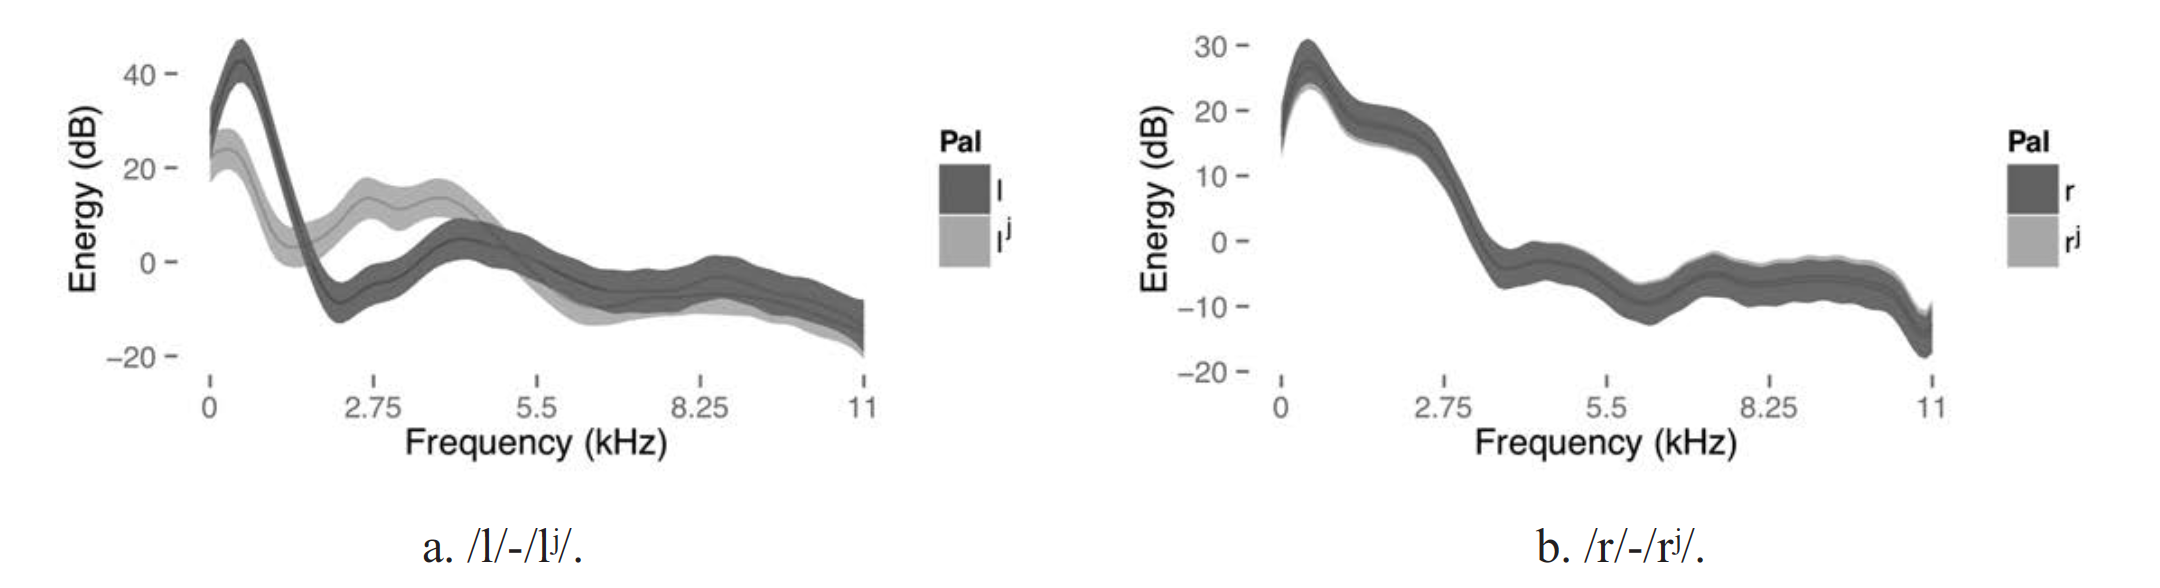
\includegraphics[width=\textwidth]{figures/a14KavitskayaWandl-img003.png}
\caption{\label{fig:kavitskaya:3} Spectral contrast for liquids in Russian; 12 speakers (\citealt{IskarousKavitskaya2018}: 60)}
\end{figure}

The absence of spectral differences between non-palatalized and palatalized rhotics is truly unexpected since the contrast between these two segments is quite robust in Russian. \citet{IskarousKavitskaya2018} propose that the explanation for why the spectral differences are leveled out when a considerable number of speakers are pooled together lies in the great variability of Russian rhotics. On the contrary, the laterals [l] and [lʲ] do not vary considerably across individuals, and thus continue to be distinguishable across speakers. While the formant transitions provide ample evidence for phonological contrast in both cases, the spectra in \figref{fig:kavitskaya:3} show that the learner is presented with a much more difficult task in discerning the palatalization contrast for the rhotics than for the laterals if the learning is exemplar-based and the available tokens are pooled together. When a learner is presented with highly variable tokens of sounds, which are phonologically contrastive but not distinct enough across speakers, the acquisition of these sounds may be impeded.

Interestingly, \citet{IskarousKavitskaya2018} show that a similar overlap in the inter-speaker spectra occurs only in the coronal fricatives /s/ : /sʲ/, /z/ : /zʲ/ and in the labials /p/ : /pʲ/, /b/ : /bʲ/, and /m/ : /mʲ/. Palatalized labials are generally considered unstable and usually occur only if a language has other palatalized consonants (\citealt{Hock2006,Bateman2011}). For instance, in Slavic we find palatalized labials in a conservative variant of Polish, which otherwise exhibits secondary palatalization contrast only in velars. The same is true for a conservative variant of Lower Sorbian, which does not have a full-fledged correlation of secondary palatalization. This can be explained by the fact that these systems present an intermediate stage in the general loss of contrastive palatalization \citep[33 ff.]{Stadnik2002}. The innovative consonant inventories of both varieties do not contain palatalized consonants anymore. In Polish, palatalized labials were retained because, unlike the palatalized coronals and velars, labials do not have an option to undergo a change of the primary place of articulation. In this regard, they are similar to the palatalized rhotic [rʲ] (see \citealt{WandlKavitskaya2023}). The prediction that /s/ and /sʲ/ contrast is less stable due to the minimal spectral difference also holds. While the /s/ : /sʲ/ contrast arose in East and South Slavic as a result of the Common Slavic velar palatalizations (the so-called Second and Third palatalizations), it is also preserved only in the languages which developed secondary palatalization of *\textit{s} before front vowels. This suggests a possibility of a correlation between the differences in the spectral contrast of plain and palatalized consonants and the contrast’s resistance to loss, along the lines of the explanation proposed by \citet{IskarousKavitskaya2018}.


Future work on the acquisition of rhotics might shed further light on the fate of the /r/ : /rʲ/ contrast in Slavic with respect to the functional and phonetic pressures that affect the contrast. There are several predictors of the relative timing of a child’s acquisition of a sound. The articulatory complexity of a sound plays a role, and the other important predictors are frequency of occurrence (\citealt{Boysson-BardiesVihman1991,Ellis2002,EdwardsBeckman2008,EdwardsEtAl2015}) and functional load (\citealt{Hockett1955,Hockett1967,WedelEtAl2013a,Cychosz2017}, among others). We have also hypothesized that intra-speaker variability may be yet another predictor. These topics remain to be investigated for the Slavic languages.

\section{Conclusion}
\label{sec:kavitskaya:6}
To conclude, we discussed the rare /r/ : /rʲ/ contrast which is present in several Slavic languages. We showed that, while the contrast can be reconstructed to Common Slavic, it has been preserved only in those Slavic languages which acquired the additional palatalization contrasts in positions other than the original jotation context. We argued that this correlation is not coincidental and proposed that functional pressures are crucial for the contrast preservation. The palatalized rhotic /rʲ/ introduced into Slavic due to yod palatalization was preserved as a reflex other than /r/ only in the languages which developed further palatalized rhotics due to the overall palatalization of consonants before front vowels. We then looked into the development of the secondary palatalization contrast in rhotics in the individual Slavic languages and addressed the phonetic factors that contributed to the survival of this rare and unstable contrast, as well as provided some discussion of the acquisition of contrast. This study has demonstrated the relevance and importance of diachronic, phonetic, functional, and acquisitional factors in the explanation of contrast preservation and loss.

\section*{Acknowledgments}

We thank the audience of the 50th Poznań Linguistic Meeting, the editors of the volume, and the anonymous reviewers for their comments and suggestions.

\section*{Abbreviations}
\begin{tabularx}{.45\textwidth}{lQ}
BCS & Bosnian/Croatian/Serbian \\
BRu & Belarusian               \\
Bu  &Bulgarian                 \\
Cz  &Czech                     \\
\textsc{gen} & genitive        \\
Mak & Macedonian               \\
\textsc{nom} & nominative      \\
\textsc{n} &  neuter      \\
\end{tabularx}
\begin{tabularx}{.45\textwidth}{lQ}
Po & Polish               \\
\textsc{prs} &  present   \\
PSl &  Proto-Slavic       \\
Ru  &Russian              \\
\textsc{sg}&  singular    \\
Slk  &Slovak              \\
Sln  &Slovenian           \\
Ukr  &Ukrainian           \\
\end{tabularx}

\sloppy\printbibliography[heading=subbibliography,notkeyword=this]
\end{document}
